\tableofcontents
\section{Introduction}

Transport investigation in strongly correlated materials out of equilibrium is a convenient way of controlling their properties and can lead to discover unexpected physics. One manifestation of strong correlations is the Mott insulator.
Mott insulator is a clear example of strong correlations where doubly occupied sites play the role of carriers. This causes a big interest in the study of doublon dynamics in experimental and theoretical works due to development of the ultrafast time-resolved experimental techniques.
There are exist ways to change the number of doublons in such materials are doping or pumping of the sample by laser pulse. 

In work of [Hideo] described how the double occupancy changes with in the magnitude of the vector potential, which leads to a change in the sign of the Coulomb interaction. 

In this paper, we want to discuss how the doublone-doublone interaction depends on the magnitude of the external electric field. 





\FloatBarrier
\section{Model and method}
The Hamiltonian of the driven half-filled Hubbard model is
\begin{equation}
\begin{split}
H(t)&=\sum_{ij,\sigma}t_{ij}{\rm exp}{\left( -i\int_{{\bf R}_{j}}^{{\bf R}_{i}}d{\bf r} \cdot {\bf A}(t) \right)}c_{i \sigma}^{\dagger}c_{j \sigma}\\
&{+U{\sum_{i} \left(n_{i \uparrow}-\frac{1}{2}\right) \left(n_{i \downarrow}-\frac{1}{2} \right)}},
\end{split}
\end{equation}

where $t_{ij}$ are electron hopping amplitudes between sites $i$ and $j$, $c^\dagger_{i\sigma}$ the creation operator for an electron of spin $\sigma$ at site $i$, $U$ the on-site interaction, $n=c^\dagger c$ the number operator. Time-dependent double occupancy defined as $d(t)= \left\langle  {n}_{\uparrow}(t) {n}_{\downarrow}(t) \right\rangle $.  To solve the model we use the nonequilibrium dynamical mean field theory (DMFT) \cite{RevModPhys_NEDMFT} in combination with a weak coupling perturbative impurity solver (iterative perturbation theory (IPT)) \cite{RevModPhys_DMFT,Damping_of_BO}. We consider an 2D square lattice with dispersion law $\varepsilon({\bf k},t)=2t\left[{\rm cos}(k_x+A_x(t))+{\rm cos}(k_y+A_y(t))\right]$ and apply the electric field along the diagonal. In a gauge with pure vector potential $A(t)$, the electric field $E(t)=-\partial_t A(t)$ enters the calculation as a time-dependent shift of the noninteracting dispersion, $\epsilon_k\rightarrow \epsilon_{k-A(t)}$. We start at $t$ = 0 in the equilibrium state at inverse temperature $\beta$=5 and switch on the vector potential as it shown in Fig. \ref{fig:Pulse_21_10}.
\FloatBarrier



\FloatBarrier
\section{Shift of the Hubbard bands}

 
\begin{figure}[h!]
\begin{minipage}[h]{0.5\linewidth}
\center{\includegraphics[width=1\linewidth]{./figure/Pulse_21.eps}} (a) \\
\end{minipage}
\hfill
\begin{minipage}[h]{0.5\linewidth}
\center{\includegraphics[width=1\linewidth]{./figure/Pulse_10.eps}} \\(b)
\end{minipage}
\caption{Pulse (a)21, (b)10.}
\label{fig:Pulse_21_10}
\end{figure}





\begin{figure}[h!]
\begin{minipage}[h]{0.5\linewidth}
\center{\includegraphics[width=1\linewidth]{./figure/docc_time_w21.eps}} (a) \\
\end{minipage}
\hfill
\begin{minipage}[h]{0.5\linewidth}
\center{\includegraphics[width=1\linewidth]{./figure/docc_time_w10.eps}} \\(b)
\end{minipage}
\caption{docc}
\label{fig:docc time w21_10}
\end{figure}





\begin{figure}[h!]
\begin{minipage}[h]{0.5\linewidth}
\center{\includegraphics[width=1\linewidth]{./figure/Etot_time_w21.eps}} (a) \\
\end{minipage}
\hfill
\begin{minipage}[h]{0.5\linewidth}
\center{\includegraphics[width=1\linewidth]{./figure/Etot_time_w10.eps}} \\(b)
\end{minipage}
\caption{Etot}
\label{fig:Etot time w21_10}
\end{figure}




\begin{figure}[h!]
\begin{minipage}[h]{0.5\linewidth}
\center{\includegraphics[width=1\linewidth]{./figure/DOS_21.eps}} (a) \\
\end{minipage}
\hfill
\begin{minipage}[h]{0.5\linewidth}
\center{\includegraphics[width=1\linewidth]{./figure/DOS_10.eps}} \\(b)
\end{minipage}
\caption{DOS}
\label{fig:DOS w21_10}
\end{figure}



\begin{figure}[h!]
\begin{minipage}[h]{0.5\linewidth}
\center{\includegraphics[width=1\linewidth]{./figure/DOS_21_small.eps}} (a) \\
\end{minipage}
\hfill
\begin{minipage}[h]{0.5\linewidth}
\center{\includegraphics[width=1\linewidth]{./figure/DOS_10_small.eps}} \\(b)
\end{minipage}
\caption{DOS small}
\label{fig:DOS small w21_10}
\end{figure}





\begin{figure}[h!]
\begin{minipage}[h]{0.5\linewidth}
\center{\includegraphics[width=1\linewidth]{./figure/docc.eps}} (a) \\
\end{minipage}
\hfill
\begin{minipage}[h]{0.5\linewidth}
\center{\includegraphics[width=1\linewidth]{./figure/E_tot.eps}} \\(b)
\end{minipage}
\caption{docc Etot}
\label{fig:docc_Etot}
\end{figure}






\begin{figure}[h!]
\begin{minipage}[h]{0.5\linewidth}
\center{\includegraphics[width=1\linewidth]{./figure/omega.eps}} (a) \\
\end{minipage}
\hfill
\begin{minipage}[h]{0.5\linewidth}
\center{\includegraphics[width=1\linewidth]{./figure/DOS_max.eps}} \\(b)
\end{minipage}
\caption{DOS peak}
\label{fig:DOS_peak}
\end{figure}





\FloatBarrier
\section{Dispersion of doublons}



\begin{figure}[h!]
\begin{minipage}[h]{0.5\linewidth}
\center{\includegraphics[width=1\linewidth]{./figure/chi_pp_loc}} (a) \\
\end{minipage}
\hfill
\begin{minipage}[h]{0.5\linewidth}
\center{\includegraphics[width=1\linewidth]{./figure/chi_ch_loc}} \\(b)
\end{minipage}
\caption{CHI loc pp ch}
\label{fig:CHI_loc_pp_ch}
\end{figure}



\begin{figure}[h!]
\begin{minipage}[h]{0.5\linewidth}
\center{\includegraphics[width=1\linewidth]{./figure/Apic_band_pp_1275_n_05_Ax_2157.png}} (a) \\
\end{minipage}
\hfill
\begin{minipage}[h]{0.5\linewidth}
\center{\includegraphics[width=1\linewidth]{./figure/Apic_band_pp_1275_n_05_Ax_2333.png}} \\(b)
\end{minipage}
\begin{minipage}[h]{0.5\linewidth}
\center{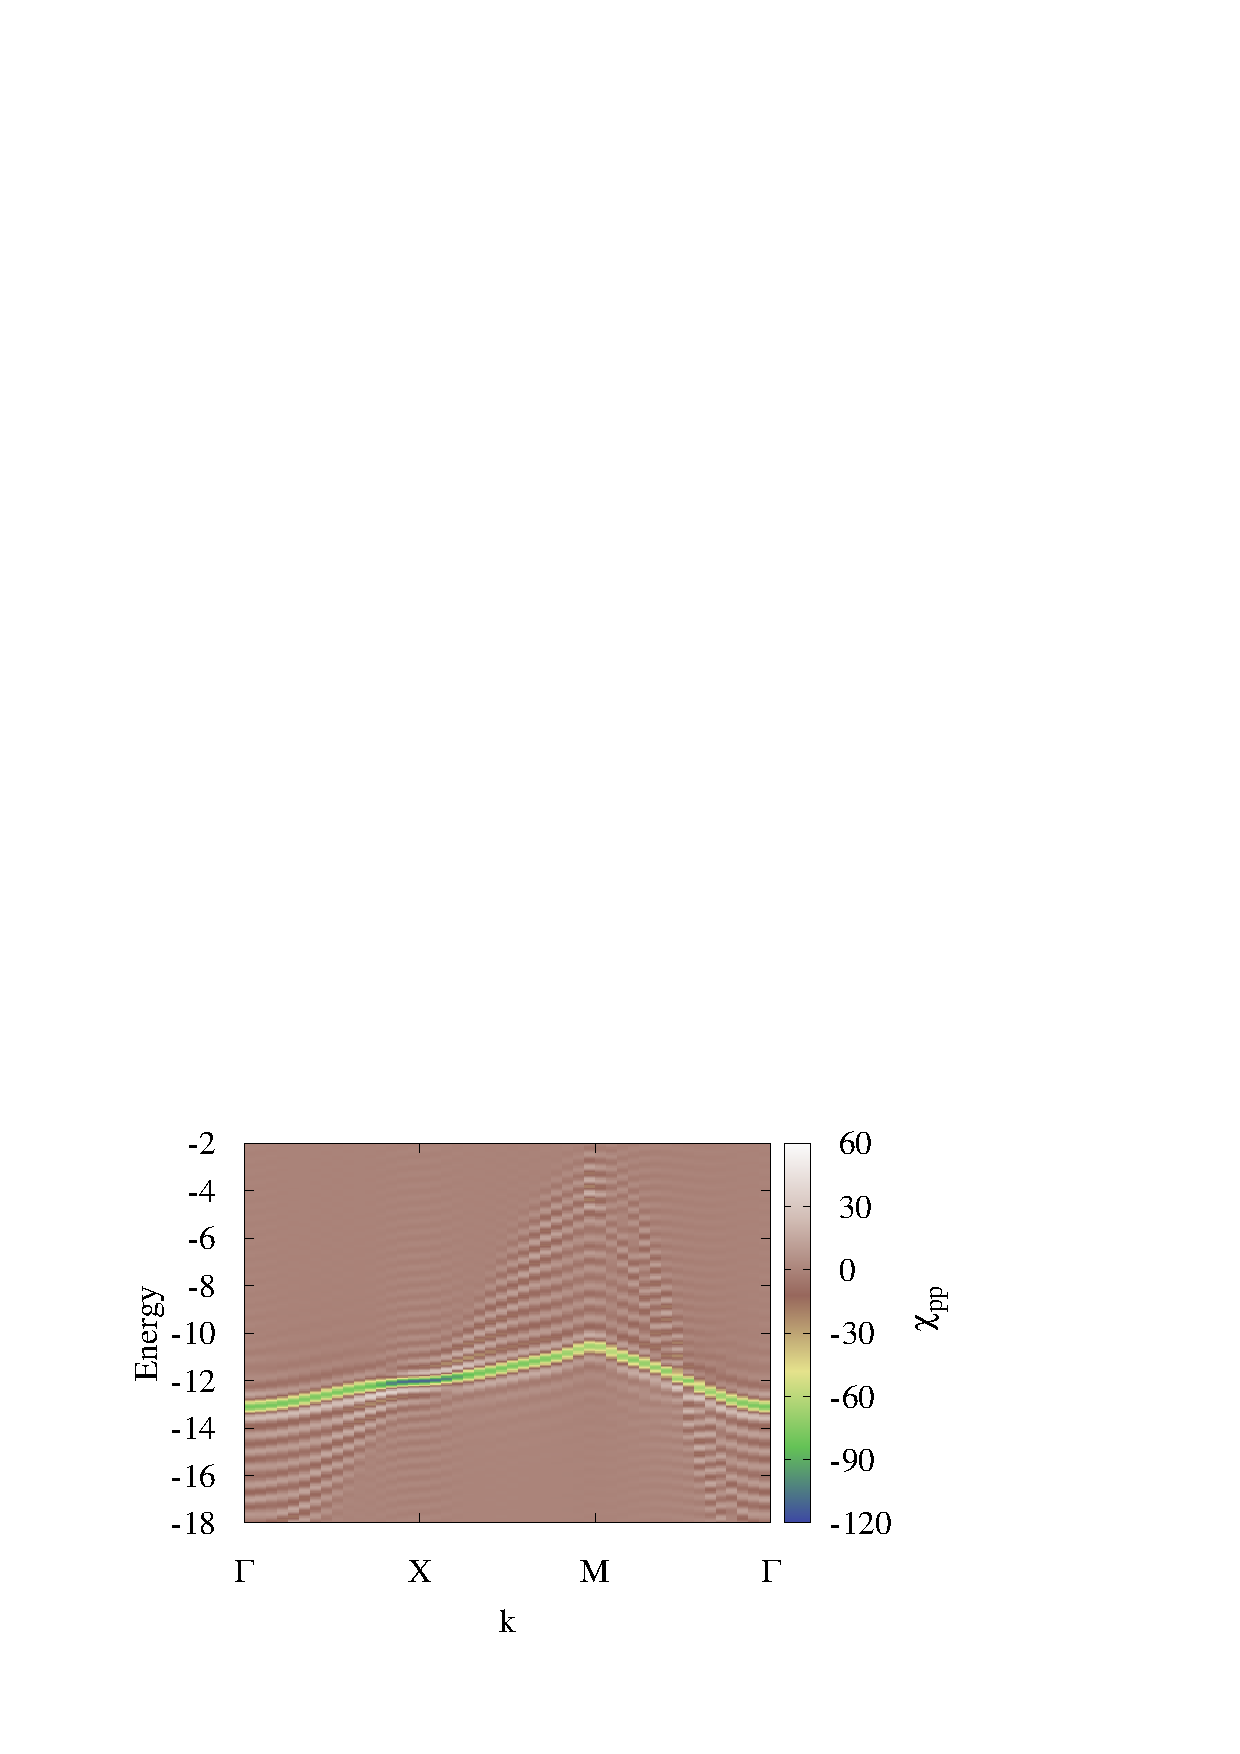
\includegraphics[width=1\linewidth]{./figure/Apic_band_pp_1275_n_1_Ax_2157.png}} (c) \\
\end{minipage}
\hfill
\begin{minipage}[h]{0.5\linewidth}
\center{\includegraphics[width=1\linewidth]{./figure/Apic_band_pp_1275_n_1_Ax_2333.png}} \\(d)
\end{minipage}
\caption{CHI k pp. $A$-dependence. (a) $A_x=2.157$ $n=0.5$, (b) $A_x=2.333$ $n=0.5$, (c) $A_x=2.157$ $n=1$, (d) $A_x=2.333$ $n=1$.}
\label{fig:CHI_k_pp_A}
\end{figure}







\begin{figure}[h!]
\begin{minipage}[h]{0.5\linewidth}
\center{\includegraphics[width=1\linewidth]{./figure/Apic_band_pp_1275_n_05_Ax_2157.png}} (a) \\
\end{minipage}
\hfill
\begin{minipage}[h]{0.5\linewidth}
\center{\includegraphics[width=1\linewidth]{./figure/Apic_band_ch_1275_n_05_Ax_2157.png}} \\(b)
\end{minipage}
\begin{minipage}[h]{0.5\linewidth}
\center{\includegraphics[width=1\linewidth]{./figure/Apic_band_pp_1275_n_0875_Ax_2157.png}} (c) \\
\end{minipage}
\hfill
\begin{minipage}[h]{0.5\linewidth}
\center{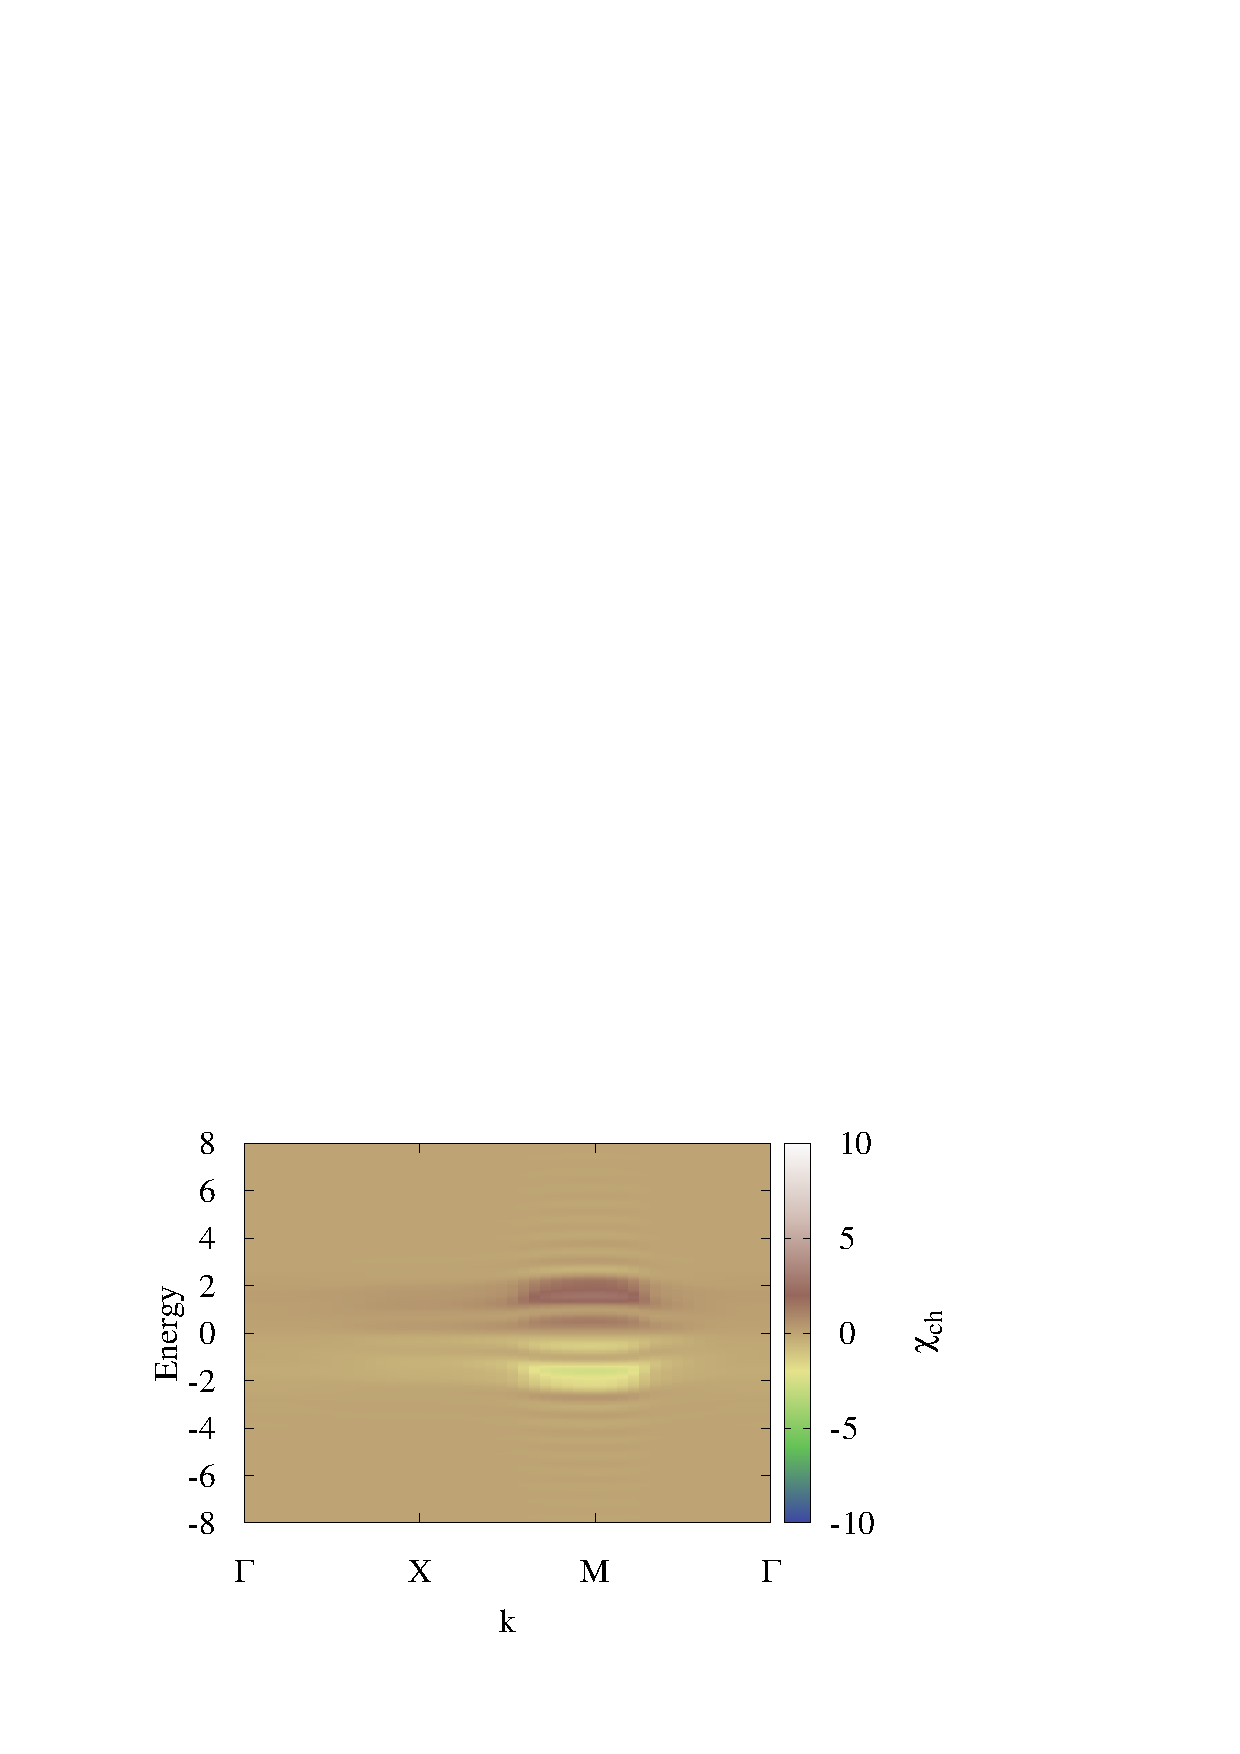
\includegraphics[width=1\linewidth]{./figure/Apic_band_ch_1275_n_0875_Ax_2157.png}} \\(d)
\end{minipage}
\begin{minipage}[h]{0.5\linewidth}
\center{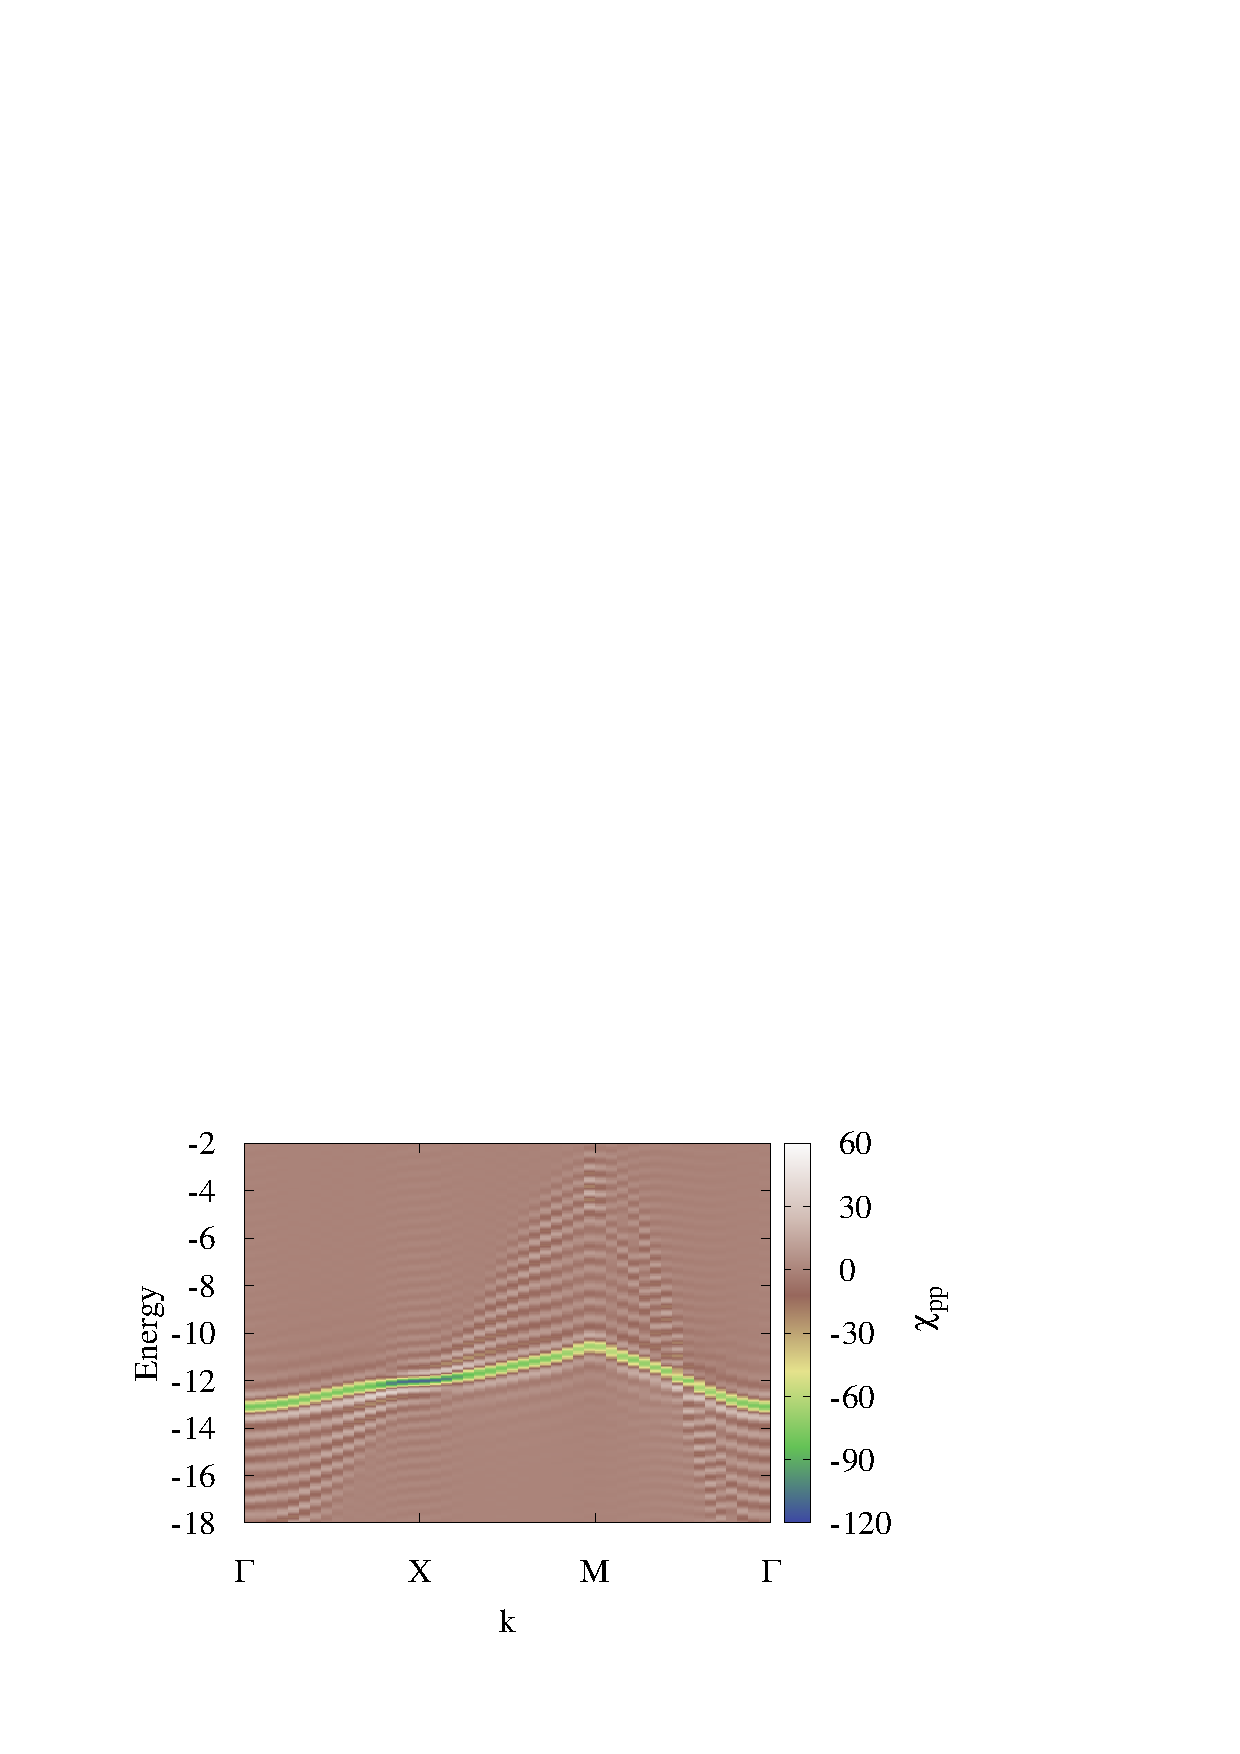
\includegraphics[width=1\linewidth]{./figure/Apic_band_pp_1275_n_1_Ax_2157.png}} (e) \\
\end{minipage}
\hfill
\begin{minipage}[h]{0.5\linewidth}
\center{\includegraphics[width=1\linewidth]{./figure/Apic_band_ch_1275_n_1_Ax_2157.png}} \\(f)
\end{minipage}
\caption{CHI k pp. $\mu$-dependence, $A_x=2.157$. (a) $\chi_{pp}$ $n=0.5$, (b) $\chi_{ch}$ $n=0.5$, (c) $\chi_{pp}$ $n=0.875$, (d) $\chi_{ch}$ $n=0.875$, (e) $\chi_{pp}$ $n=1$, (f) $\chi_{ch}$ $n=1$.}
\label{fig:CHI_k_pp_mu}
\end{figure}






\FloatBarrier
\section{Summary}














\FloatBarrier